\documentclass[a4j,10pt,dvipdfmx]{jarticle}
\usepackage{url}
\usepackage[version=3]{mhchem}
\usepackage{siunitx}
\usepackage[dvipdfmx]{graphicx}
\usepackage{pdfpages}
\usepackage{here}
\usepackage{tabularx}
\author{学籍番号2120029, 氏名 政野玄空}
\date{2023年6月17日}
\begin{document}
\title{事前課題}
\maketitle
\section{1.反転増幅回路について、回路図上に必要変数を示し、入力電圧Vi と出力電圧Vo の関
係から数式と説明文で電圧増幅率AV を導出し、説明する。 
  入出力電圧の他、入力抵抗R1 や帰還抵抗R2 に流れる電流 I1, I2 を仮定し、バーチャ
ルショートの概念から各部の電位を把握するとよい。必要に応じて参考文献を参照
する。 }
オペアンプは内部のモジュール回路の作用により,2つの入力端子の電位差が生じないようになっている.このことをバーチャルショートと呼ぶ.
\begin{figure}[H]
  \begin{center}
  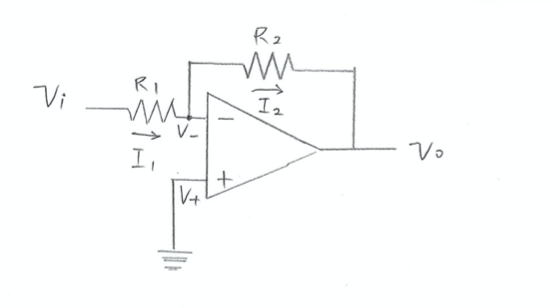
\includegraphics[height=7cm,width=10cm]{hanpuku.png}
  \caption{反転動作回路}
\end{center}
\end{figure}
バーチャルショートを保つことより,$V_-$と$V_+$は等しい.入力インピーダンスが高いため$R_1$を通った電流はすべて$R_2$に流れる.よって$R_1$に流れる電流と$R_2$に流れる電流は等しい.
よって
\begin{eqnarray}
  \label{icib}
\frac{{V_i}-{V_-}}{R_1} = \frac{{V_-}-{V_o}}{R_2} 
\end{eqnarray}
\begin{eqnarray}
  \label{Av}
A_V=\frac{V_o}{V_i} = -\frac{R_2}{R_1} 
\end{eqnarray}
となる.
\section{2.非反転増幅回路について回路図を示し、1.と同様に行う。}
1.と同様に$V_-$と$V_+$は等しい.
\begin{figure}[H]
  \begin{center}
  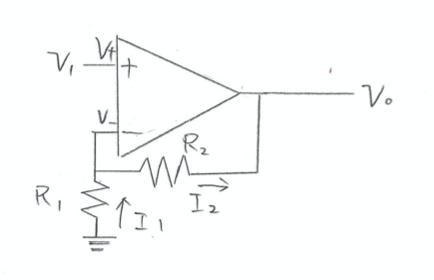
\includegraphics[height=7cm,width=10cm]{hiha.png}
  \caption{非反転動作回路}
  \label{res3-2}
\end{center}
\end{figure}
図:非反転動作回路より$R_1$を通った電流は入力インピーダンスが高いためすべて$R_2$に流れる.$V_-$の電位は$V_o$を抵抗で分圧して
\begin{eqnarray}
  \label{vvvv}
V_-=V_{o}\frac{R_1}{R_1+R_2}
\end{eqnarray}
よって
\begin{eqnarray}
  \label{Av2}
A_V=\frac{V_o}{V_i} = 1+\frac{R_2}{R_1} 
\end{eqnarray}
となる.

\section{3.加算回路について、反転増幅回路の式を参考にして出力電圧の式(3.3)を導出する。回
路図上に必要変数を示し適宜定義しておく。加算回路では入力抵抗R1, R2 や帰還抵抗
Rf に流れる電流I1, I2, If を仮定し、反転増幅回路と同様にバーチャルショートの概念
を適用して各部の電位を把握する。 }
同様に$V_-$と$V_+$は等しい.
\begin{figure}[H]
  \begin{center}
  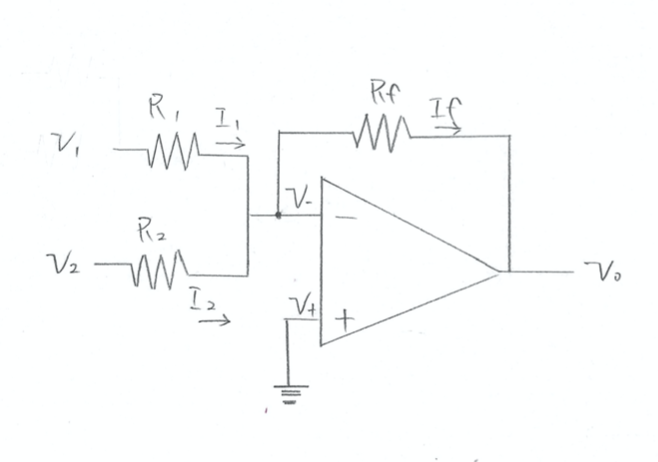
\includegraphics[height=7cm,width=10cm]{kasan.png}
  \caption{加算回路}
\end{center}
\end{figure}
加算回路は,反転増幅回路の入力を2つにしたものと考えることができるので,$R_1$と$R_2$の電流を一旦$R_{12}$とし,,$V_1$と$V_2$を$V_i$とおく.
1.と同様に入力インピーダンスが高いため$R_{12}$を通った電流はすべて$R_f$に流れる.よって$R_{12}$に流れる電流と$R_f$に流れる電流は等しい.
\begin{eqnarray}
  \label{vvvvvvvv}
\frac{{V_i}-{V_-}}{R_{12}} =  \frac{{V_-}-{V_o}}{R_f} 
\end{eqnarray}
$R_{12}$を$R_1$と$R_2$に戻すと
  \begin{eqnarray}
    \label{vvvvvvvvv}
  \frac{{V_1}-{V_-}}{R_1} + \frac{{V_2}-{V_-}}{R_2} =  \frac{{V_-}-{V_o}}{R_f} 
  \end{eqnarray}
  $V_+$が接地してあることより
  \begin{eqnarray}
    \label{voi}
  V_+ = V_- = 0
  \end{eqnarray}
(\ref{vvvvvvvvv})に(\ref{voi})を代入して整理すると
\begin{eqnarray}
  \label{voqi}
V_o = -(\frac{R_f}{R_1}V_1+\frac{R_f}{R_2}V_2)
\end{eqnarray}
となる.
\section{参考文献}
\begin{thebibliography}{9}
  \bibitem{a} 電気通信大学『アナログ回路実験』2023年,p23$\sim$25
\end{thebibliography}
\end{document}
